\section{Preliminaries}

\parbf{Proposed notation for trees.}
We will encode the trees using brackets.

\hide
\begin{wrapfigure}{r}{15 mm}
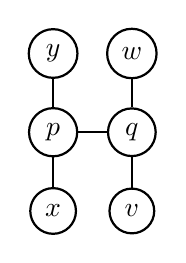
\begin{tikzpicture}[scale=1,
  thick,main node/.style={circle,draw,font=\sffamily\bfseries,minimum size=3mm}]
  \node[main node] (1) at (0,0) {$x$};
  \node[main node] (2) at (0,1){$p$};
  \node[main node] (3) at (0,2){$y$};
  \node[main node] (4) at (1,0) {$v$};
  \node[main node] (5) at (1,1) {$q$};
  \node[main node] (6) at (1,2) {$w$};

  \path[every node/.style={font=\sffamily\small}]
   (1) edge node[above]{}(2)
   (2) edge node[above]{}(3)
   (2) edge node[above]{}(5)
   (4) edge node[above]{}(5)
   (5) edge node[above]{}(6);
\end{tikzpicture}
\end{wrapfigure}
\unhide

For example $(()()(()()))$ encodes the tree with 6 vertexes on the diagram. 
One vertex for each pair of brakes;
we assume that a pair vertexes is adjacent if the corresponding pairs of brackets nested directly one into another.

We will use shortcut
\[n=\underbrace{()\dots()}_{n\text{ times}};\]
so we can write $(2(2))$ instead of $(()()(()()))$.

To encode the labelig of vertexes as on the diagram, we will use notation $p,xy(q,vw)$;
here $p$ and $q$ are connected to the first element in each group followed by comma.
Taking another root for the tree, we can write it as $q,vw(p,x,y)$ or as $x,(p,y(q,vw))$.

\begin{thm}{Kirszbraun rigidity theorem}\label{thm:kirszbraun-rigid}
Let $A$ be a complete $\CBB[0]$ length space.

Assume that for two point arrays $p,x_1,\dots,x_n\in A$ and $\~q, \~x_1,\dots,\~x_n\in \HH$ we have that 
\[|\~q-\~x_i|\ge |p-x_i|\]
for any $i$,
\[|\~x_i-\~x_j|\le |x_i-x_i|\]
for any pair $(i,j)$
and $\~q$ lies in the interior of the convex hull $K$ of $\~x_1,\dots,\~x_n$.

Then equalities hold in all the inequalities above.
Moreover there is an distance preserving map $f\:K\to A$ such that $f(\~x_i)=x_i$ and $f(\~q)=p$. 
\end{thm}

\parit{Proof.}
By the generalized Kirszbraun theorem, there is a short map $f\:A\to \HH$
such that $f(x_i)=\~x_i$.
Set  $\~p=f(p)$.
By assumptions
\[|\~q-\~x_i|\ge |\~p-\~x_i|.\]

Since $\~q$ lies in the interior of $K$, $\~q=\~p$.
It follows that the equality 
\[|\~q-\~x_i|= |p-x_i|.\]
holds for each $i$.

According to ???, there is a short map $\HH\to \T_p$ such which admits a right inverse $\T_p\to \HH$ such that ...



\qeds